% ===========================================================
%  Лекция 13. Поиск кратчайших путей во взвешенном графе
% ===========================================================

\chapter{Лекция 13. Поиск кратчайших путей во взвешенном графе}

Пусть $G(V, E)$~--- ориентированный связный (слабо) граф, $\sigma\colon E \to \mathbb{R}$~--- весовая функция.

\textbf{Пример} (рис.~p29-example-1): граф $A, B, C, D, K$ с рёбрами $AB\,(1)$, $BC\,(-2)$, $CD\,(-2)$, $DB\,(3)$, $BK\,(8)$. Цикл $B \to C \to D \to B$ имеет суммарный вес $(-2) + (-2) + 3 = -1 < 0$~--- отрицательный цикл.

\grfig{figures/p29-example-1.pdf}{Граф с отриц. циклом: A,B,C,D,K}

\textbf{Критерий} (необходимость и достаточность): кратчайшие пути существуют тогда и только тогда, когда в $G$ отсутствуют циклы отрицательного суммарного веса.

\textit{Почему.} ($\Leftarrow$) Если отрицательных циклов нет, то из
любого маршрута можно выбрасывать циклы, не увеличивая длину, --- значит,
среди кратчайших маршрутов есть \emph{простой} путь; простых путей
конечное число, и минимум достигается. ($\Rightarrow$) Если же
отрицательный цикл достижим, то, прокручивая его сколько угодно раз,
длину маршрута можно сделать сколь угодно малой --- минимума нет
(в примере выше путь $A \to B \to K$ можно «удешевлять» обходами цикла
$B \to C \to D \to B$ по $-1$ за круг).

Отдельные рёбра отрицательного веса в общем случае возможны.

\textbf{Задачи:}
\begin{enumerate}
  \item[$\oplus$] Кратчайшие пути от фиксированной вершины $v \in V$ до всех $w \in V$.
  \item[$\odot$] Кратчайшие пути для каждой пары $u, v \in V$.
\end{enumerate}

Кратчайший путь $\neq$ его длина:
\[
  S = A_0 \to A_1 \to A_2 \to \ldots \to A_k \to \ldots \to A_{n-1} \to A_n = F.
\]
$P(A_i) = A_{i-1}$ (предок), $G(A_i) = A_{i+1}$ (потомок).

% ===========================================================
%  Алгоритм Дейкстры
% ===========================================================

\begin{algo}{Алгоритм Дейкстры}{dijkstra}

\textbf{Требование:} $\sigma\colon E \to \mathbb{R}_{\geq 0}$ (только неотрицательные веса!).

\textbf{Инициализация:}
$\mu(\text{start}) := 0$, \quad $\mu(v) := \infty$ для всех остальных вершин.

\textbf{Шаг:} Выбираем $v$ с минимальной меткой $\mu(v)$ среди непосещённых.

Для каждого $w \in \mathrm{Ch}(v)$:
\[
  \text{если } \mu(w) > \mu(v) + \sigma(\overline{vw}), \text{ то }
  \begin{cases}
    \mu(w) := \mu(v) + \sigma(\overline{vw}), \\
    P(w) := v.
  \end{cases}
\]

Это \textbf{динамическое программирование} (жадный выбор + оптимальная подструктура).

\textit{Почему жадный выбор корректен:} пусть $v$ --- непосещённая
вершина с минимальной меткой $\mu(v)$. Любой путь из старта в $v$
обязан в какой-то момент впервые покинуть множество посещённых вершин по
ребру $x \to y$ ($y$ не посещена); его длина не меньше
$\mu(y) \ge \mu(v)$, а дальнейшие рёбра \emph{неотрицательны} ---
короче $\mu(v)$ не получится. Значит, метку $\mu(v)$ можно зафиксировать
как окончательную. (Именно здесь существенно $\sigma \ge 0$: с
отрицательными рёбрами «дешёвый обход позже» возможен, и жадность
ломается --- нужен Форд--Беллман.)

\textbf{Пример} (рис.~p29-djakstra-example-1): граф $A, B, C, D$. Start $= A$. Рёбра: $BA\,(2)$, $CB\,(5)$, $AC\,(10)$, $DC\,(3)$, $AD\,(2)$, $BD\,(7)$.

\grfig{figures/p29-djakstra-example-1.pdf}{Алг. Дейкстры: A,B,C,D (AD=2,AC=10,DC=3,BD=7,CB=5,BA=2)}

\begin{center}
\begin{tabular}{c|c|c|c|c}
       & $A$  & $B$      & $C$      & $D$      \\
\hline
Иниц.  & 0    & $\infty$ & $\infty$ & $\infty$ \\
$A$    & $-$  & $\infty$ & $10, A$  & $2, A$   \\
$D$    & $-$  & $\infty$ & $5, D$   & $-$      \\
$C$    & $-$  & $10, C$  & $-$      & $-$      \\
\end{tabular}
\end{center}

$D \to C$: $\mu(D) = 2$, $\sigma(DC) = 3$, итого $2 + 3 = 5 < 10$, обновляем.

Дерево кратчайших путей: $A \xrightarrow{2} D \xrightarrow{3} C \xrightarrow{5} B$.

\medskip
\noindent\textbf{Работа алгоритма по шагам.} Для разнообразия
демонстрация выполнена на другом графе (7 вершин, рис.~p9-example-0,
веса проставлены детерминированно), старт~--- $A$.
\begin{center}\begin{tabular}{ccc}
\shortstack{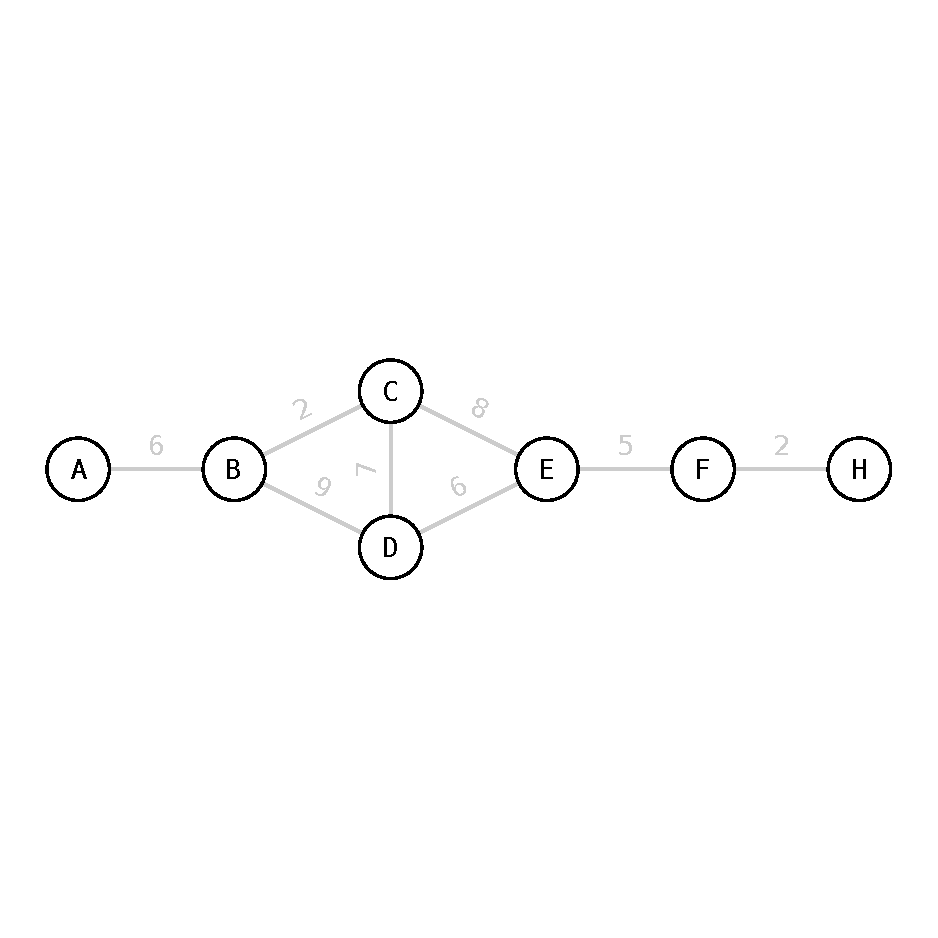
\includegraphics[width=0.28\textwidth]{python/lec13/dijkstra/dijkstra-0.pdf}\\[2pt]{\scriptsize Шаг 0}} &
\shortstack{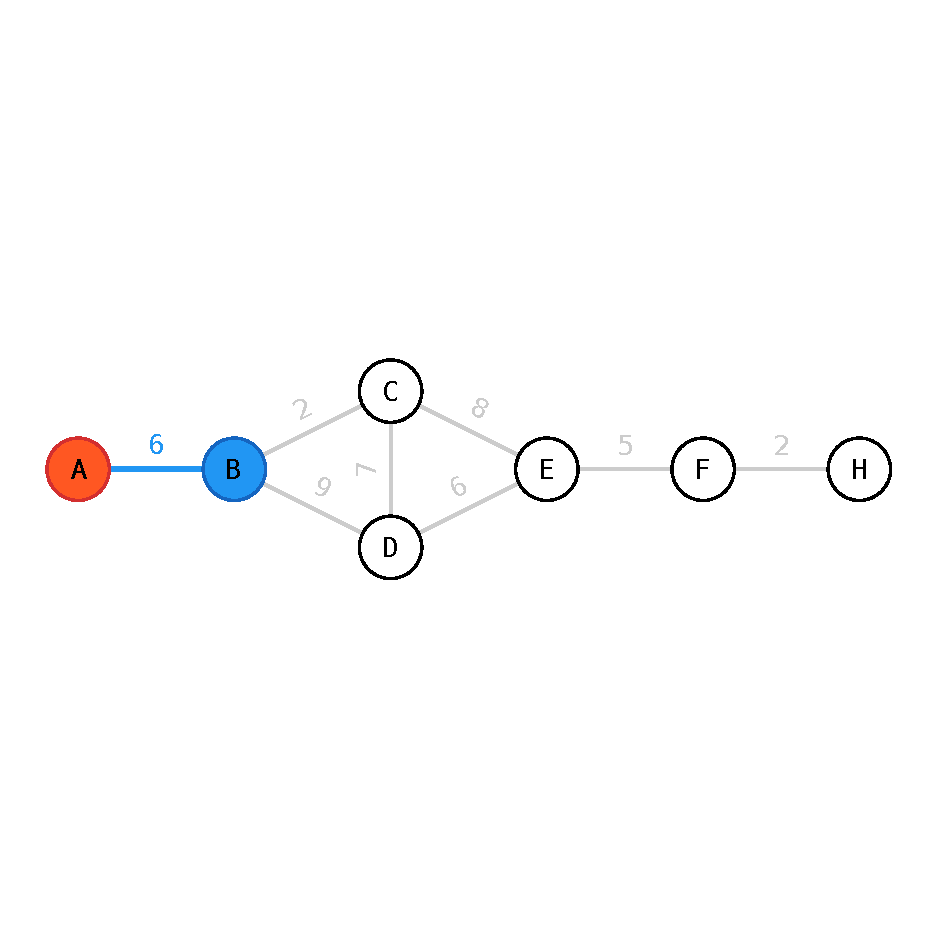
\includegraphics[width=0.28\textwidth]{python/lec13/dijkstra/dijkstra-1.pdf}\\[2pt]{\scriptsize Шаг 1}} &
\shortstack{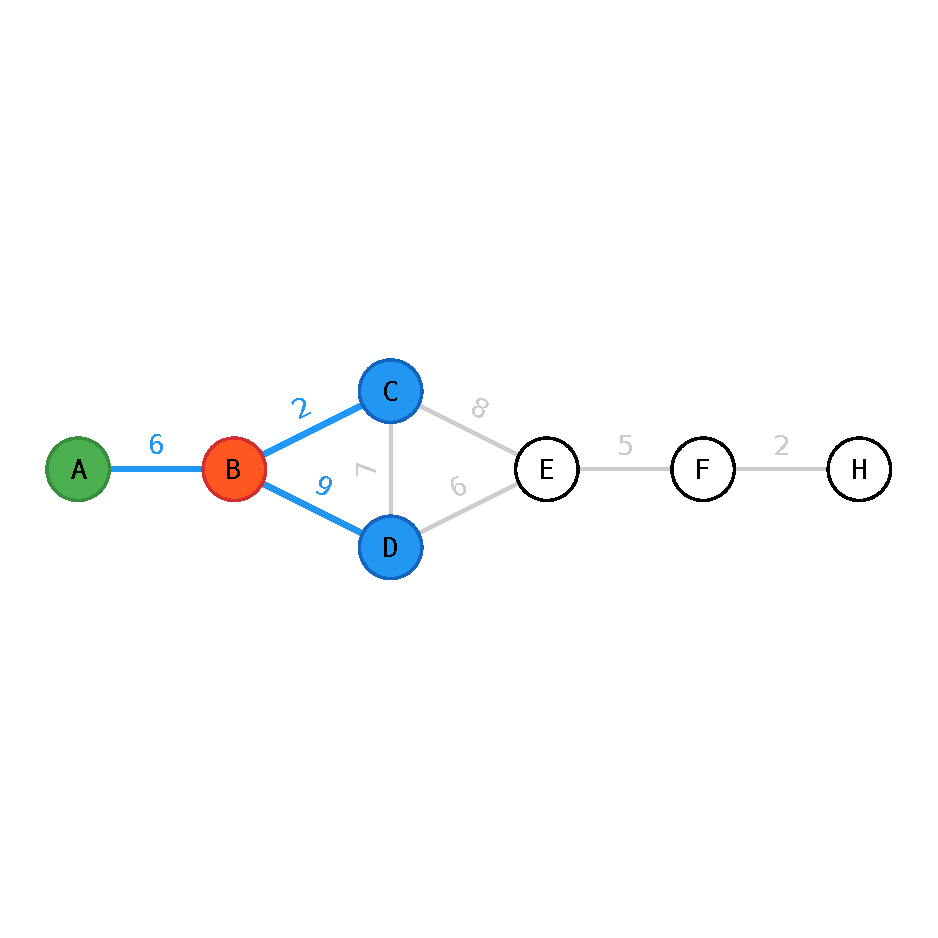
\includegraphics[width=0.28\textwidth]{python/lec13/dijkstra/dijkstra-2.pdf}\\[2pt]{\scriptsize Шаг 2}} \\
\end{tabular}\end{center}
\begin{center}\begin{tabular}{ccc}
\shortstack{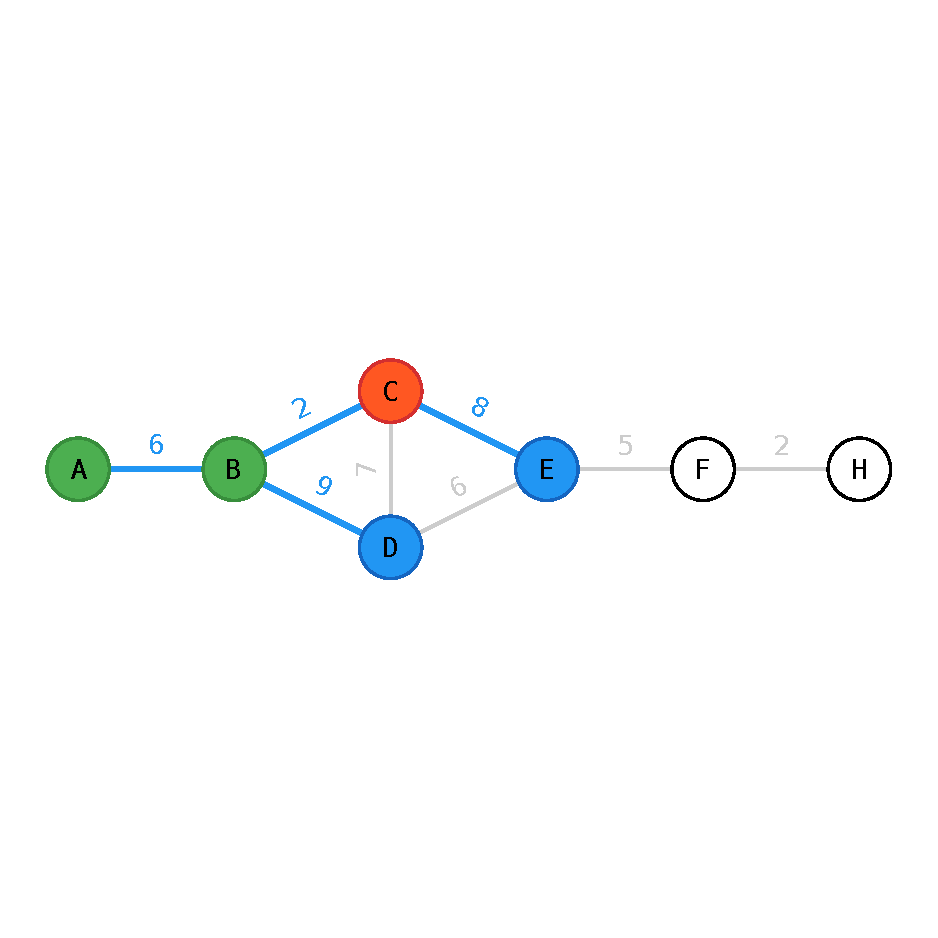
\includegraphics[width=0.28\textwidth]{python/lec13/dijkstra/dijkstra-3.pdf}\\[2pt]{\scriptsize Шаг 3}} &
\shortstack{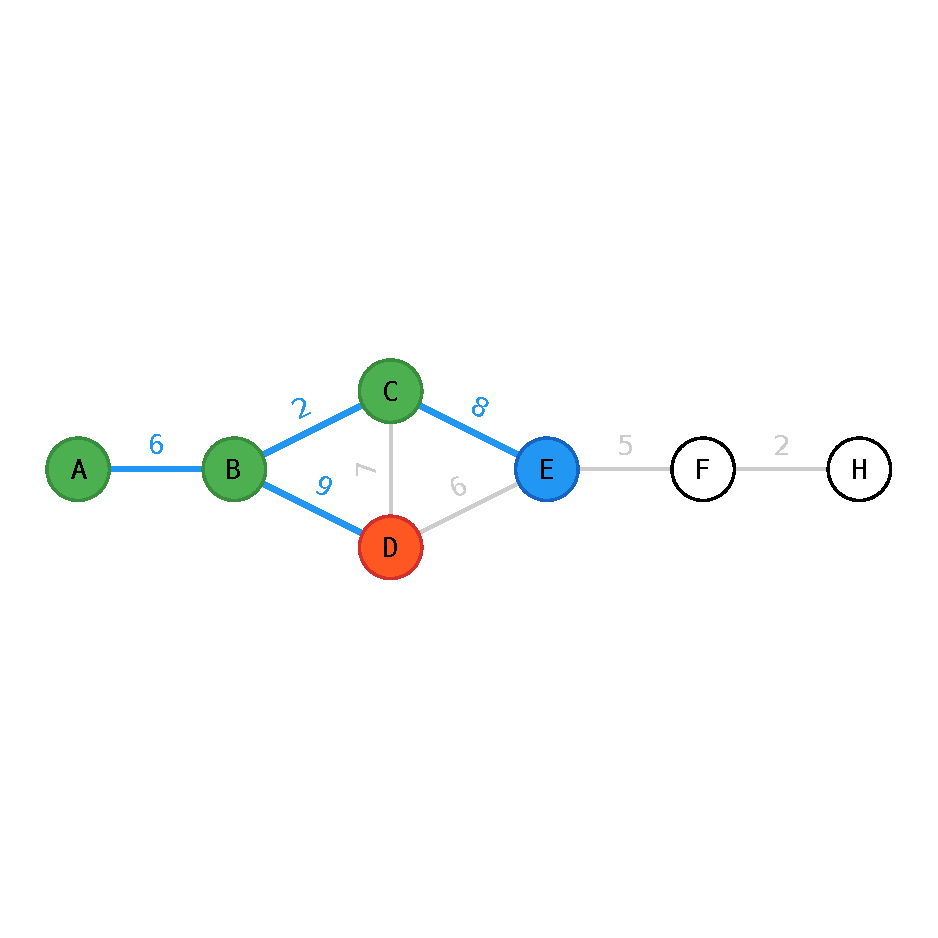
\includegraphics[width=0.28\textwidth]{python/lec13/dijkstra/dijkstra-4.pdf}\\[2pt]{\scriptsize Шаг 4}} &
\shortstack{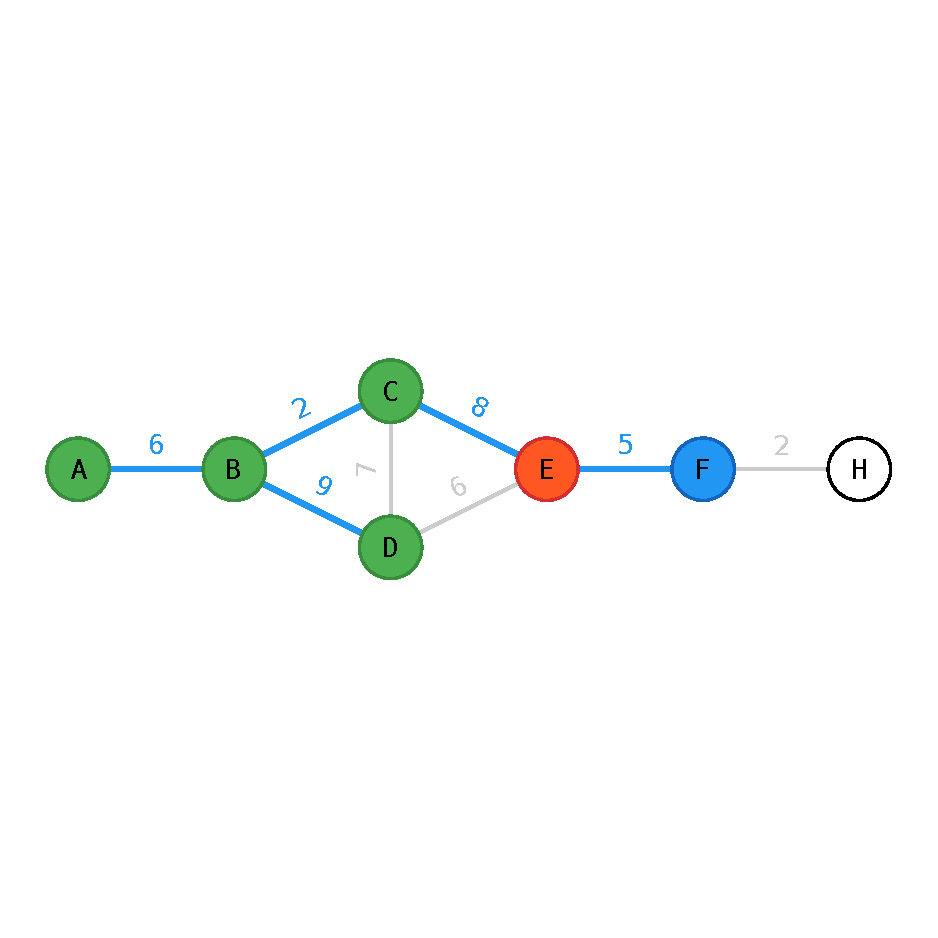
\includegraphics[width=0.28\textwidth]{python/lec13/dijkstra/dijkstra-5.pdf}\\[2pt]{\scriptsize Шаг 5}} \\
\end{tabular}\end{center}
\begin{center}\begin{tabular}{ccc}
\shortstack{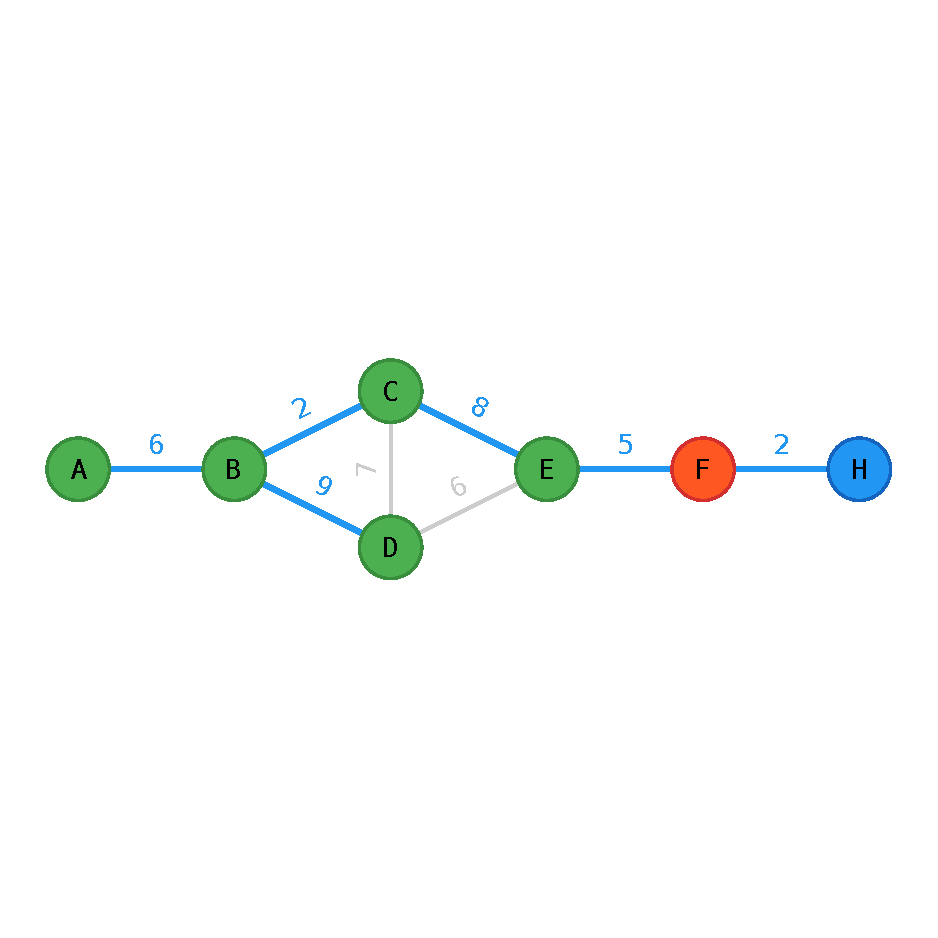
\includegraphics[width=0.28\textwidth]{python/lec13/dijkstra/dijkstra-6.pdf}\\[2pt]{\scriptsize Шаг 6}} &
\shortstack{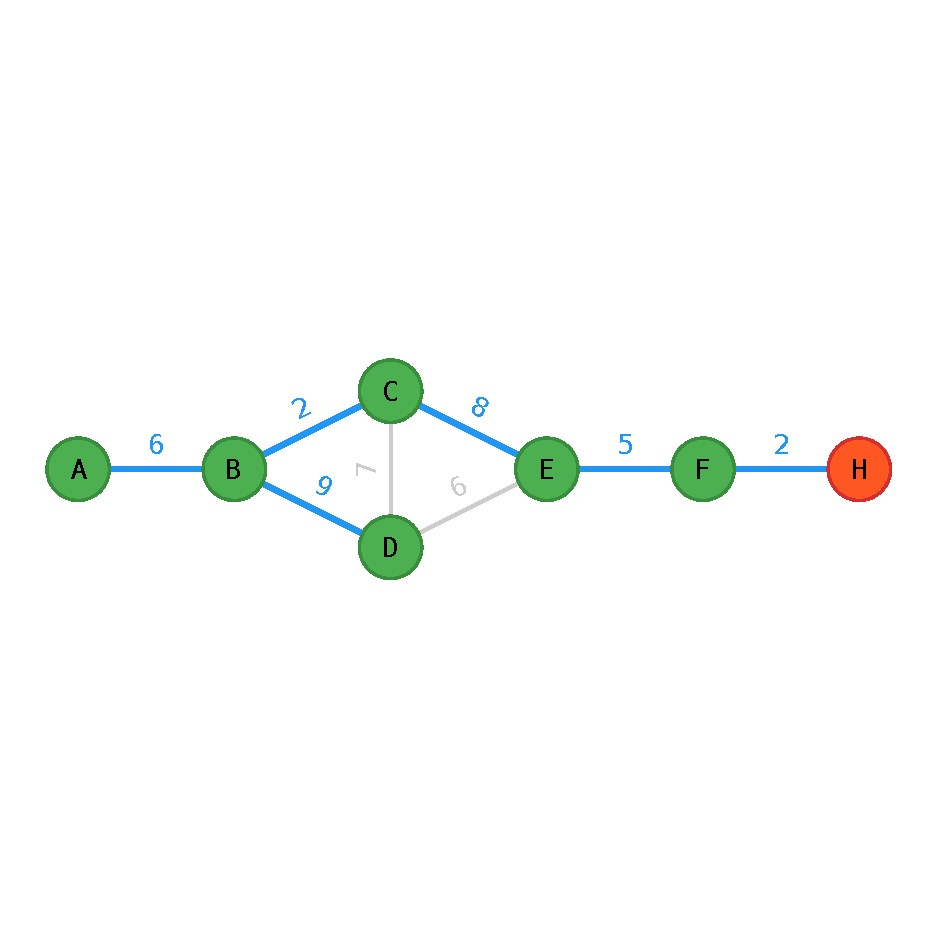
\includegraphics[width=0.28\textwidth]{python/lec13/dijkstra/dijkstra-7.pdf}\\[2pt]{\scriptsize Шаг 7}} &
\shortstack{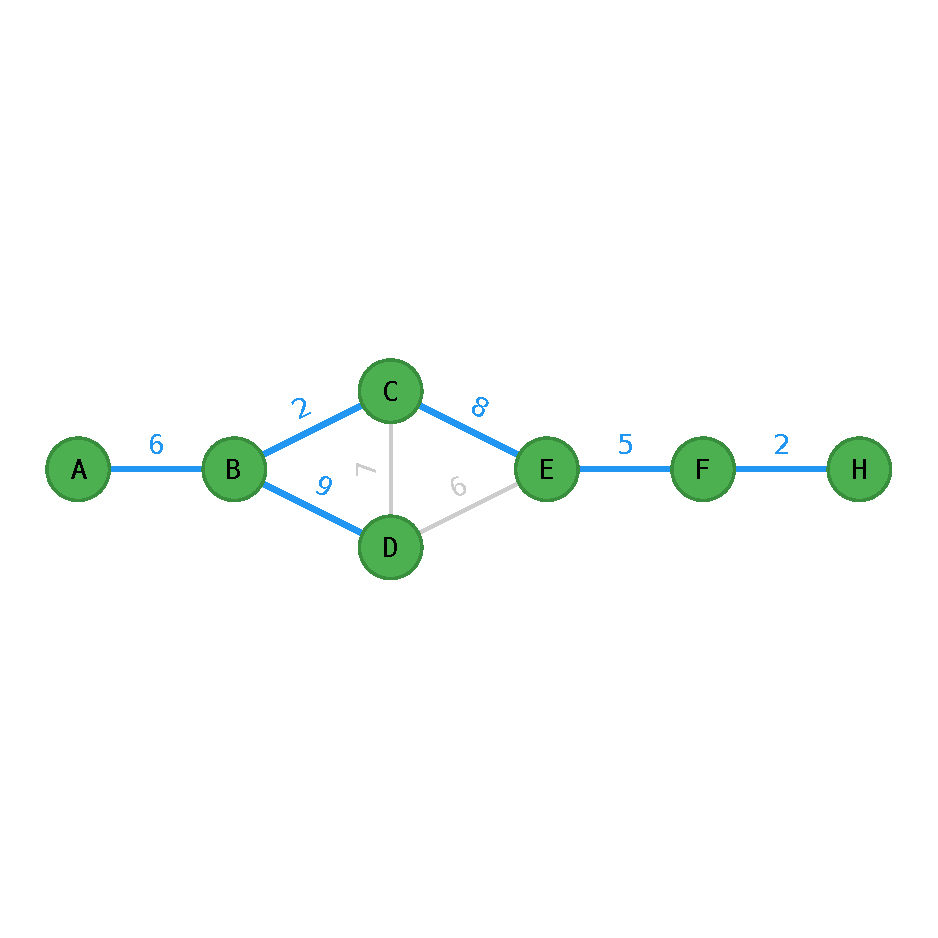
\includegraphics[width=0.28\textwidth]{python/lec13/dijkstra/dijkstra-8.pdf}\\[2pt]{\scriptsize Шаг 8}} \\
\end{tabular}\end{center}

\end{algo}

% ===========================================================
%  Алгоритм Форда-Беллмана
% ===========================================================

\begin{algo}{Алгоритм Форда-Беллмана}{ford-bellman}

\textbf{Допускается:} $\sigma\colon E \to \mathbb{R}$ (в том числе отрицательные веса).

\textbf{Инициализация:}
Произвольное упорядочивание рёбер. Стартовая вершина $v$: $\mu(v) := 0$, $\mu(w) := \infty$ для остальных.

\textbf{Шаг} (1 шаг = полный просмотр списка рёбер):

$\forall\, e_i \in \mathrm{list}(E)$, $e_i = uv$:
\[
  \text{если } \mu(v) > \mu(u) + \sigma(e_i), \text{ то }
  \begin{cases}
    \mu(v) := \mu(u) + \sigma(e_i), \\
    P(v) := u.
  \end{cases}
\]

\textbf{Конец алгоритма:} шаги $k$ и $k+1$ дают одинаковый результат. Если $n$ вершин, то алгоритм сойдётся не позже чем за $n - 1$ шагов.

\textit{Почему работает:} индукцией по $k$ проверяется инвариант ---
после $k$-го прохода по списку рёбер метка $\mu(w)$ не превосходит длины
кратчайшего пути из старта в $w$, содержащего $\le k$ рёбер (релаксация
последнего ребра такого пути произойдёт не позже $k$-го прохода).
Кратчайшие пути просты, т.\,е.\ содержат не более $n - 1$ ребра, поэтому
$n - 1$ проходов достаточно. Если же обновления случаются и на $n$-м
проходе --- в графе есть достижимый отрицательный цикл (так его и
детектируют).

\textbf{Пример} (рис.~p30-fb-example-1): граф $A, B, C, D$. Start $= B$. Отличие от Дейкстры: ребро $BA$ имеет вес $-2$.

\grfig{figures/p30-fb-example-1.pdf}{Алг. Форда-Беллмана: тот же граф, BA=-2}

Список рёбер с весами:
\begin{center}
\begin{tabular}{cc}
Ребро & Вес \\
\hline
$AC$ & 10 \\
$AD$ & 2 \\
$BA$ & $-2$ \\
$BD$ & 7 \\
$CB$ & 5 \\
$DC$ & 3 \\
\end{tabular}
\end{center}

Протокол:
\begin{center}
\begin{tabular}{c|c|c|c|c}
       & $A$    & $B$ & $C$                & $D$    \\
\hline
Иниц.  & $\infty$ & 0 & $\infty$          & $\infty$ \\
Шаг 1  & $-2, B$  & 0 & $7+3=10, D$       & $7, B$   \\
Шаг 2  & $-2, B$  & 0 & $8, A$ $\to$ $3, D$ & $0, A$   \\
\end{tabular}
\end{center}

Корневое дерево кратчайших путей: $B \xrightarrow{-2} A \xrightarrow{2} D \xrightarrow{3} C$.

\medskip
\noindent\textbf{Работа алгоритма по шагам:}
\begin{center}\begin{tabular}{ccc}
\shortstack{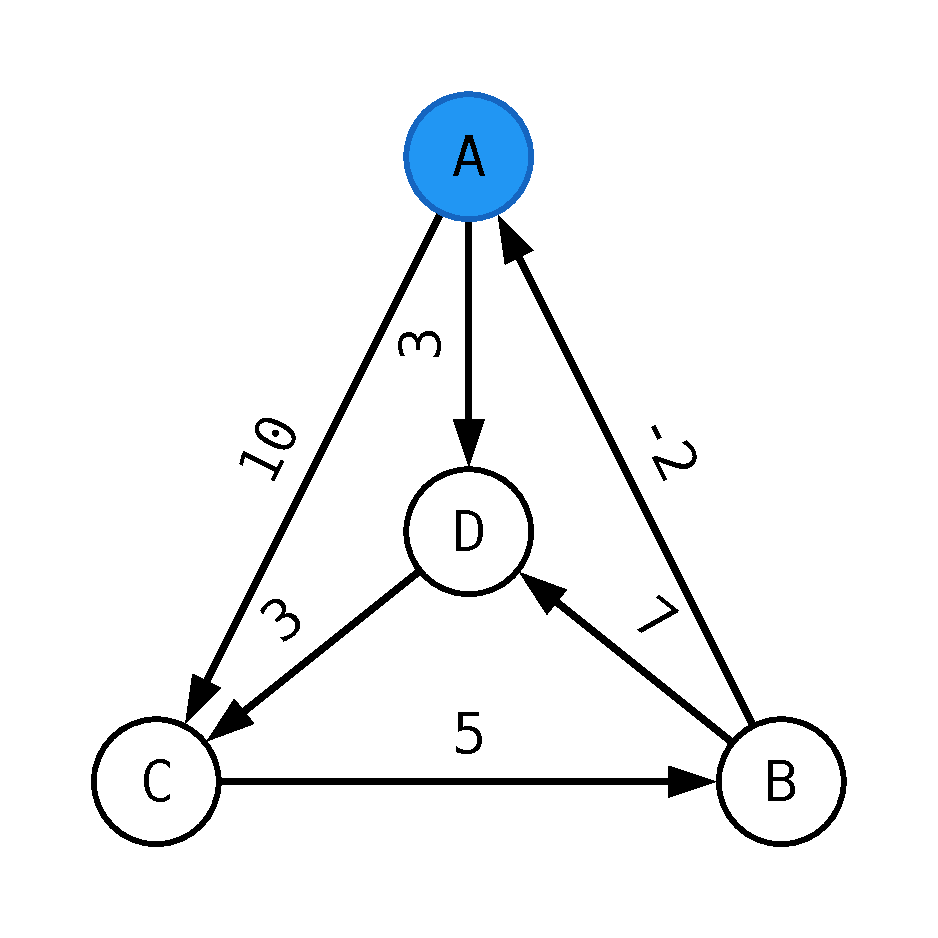
\includegraphics[width=0.28\textwidth]{python/lec13/bellman_ford/bellman_ford-0.pdf}\\[2pt]{\scriptsize Шаг 0}} &
\shortstack{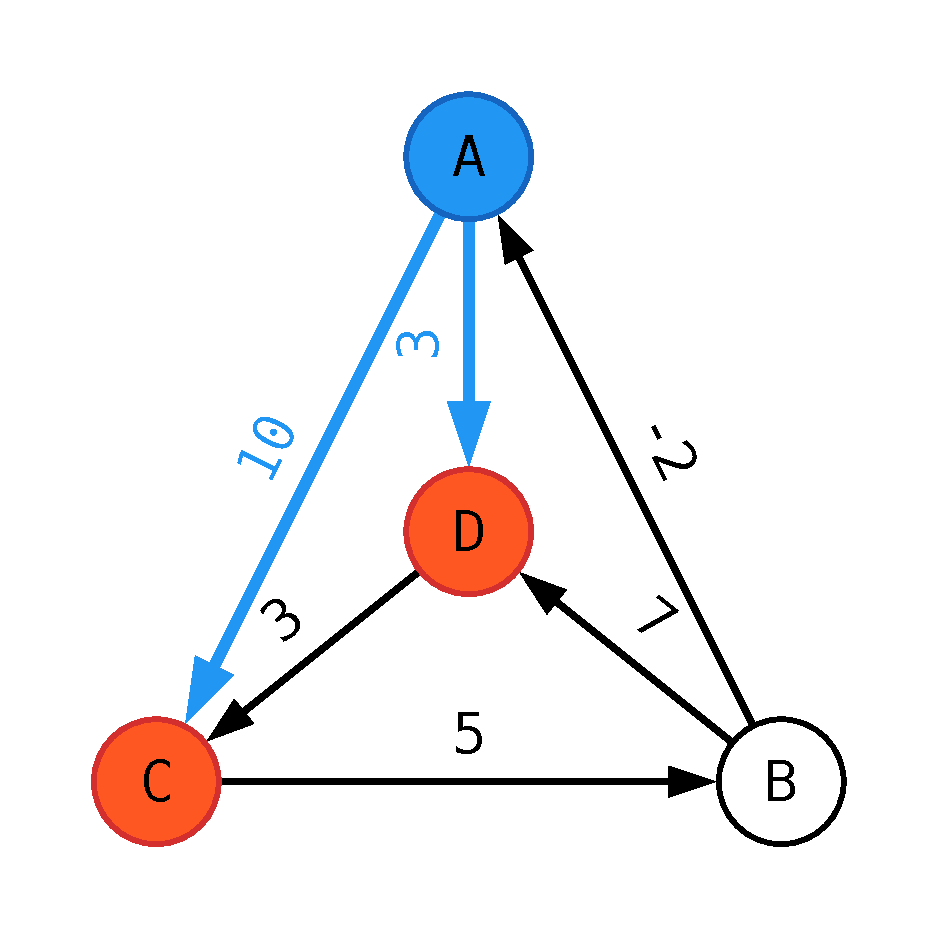
\includegraphics[width=0.28\textwidth]{python/lec13/bellman_ford/bellman_ford-1.pdf}\\[2pt]{\scriptsize Шаг 1}} &
\shortstack{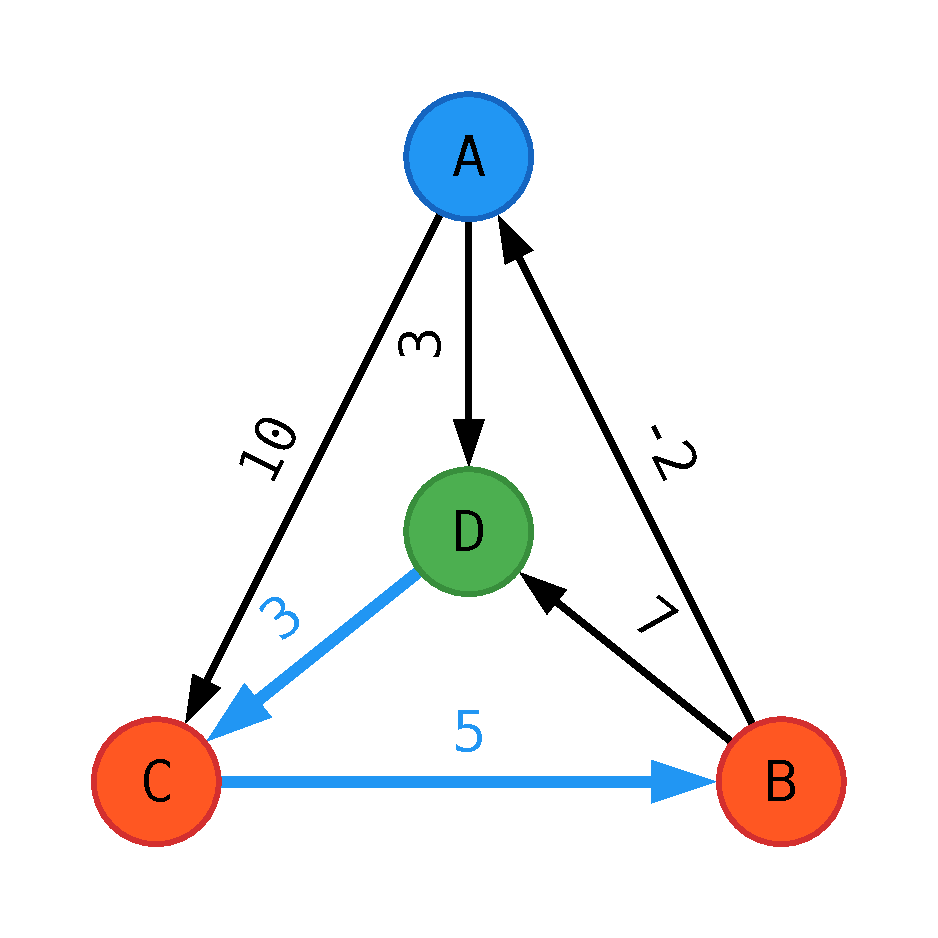
\includegraphics[width=0.28\textwidth]{python/lec13/bellman_ford/bellman_ford-2.pdf}\\[2pt]{\scriptsize Шаг 2}} \\
\end{tabular}\end{center}
\begin{center}\begin{tabular}{cc}
\shortstack{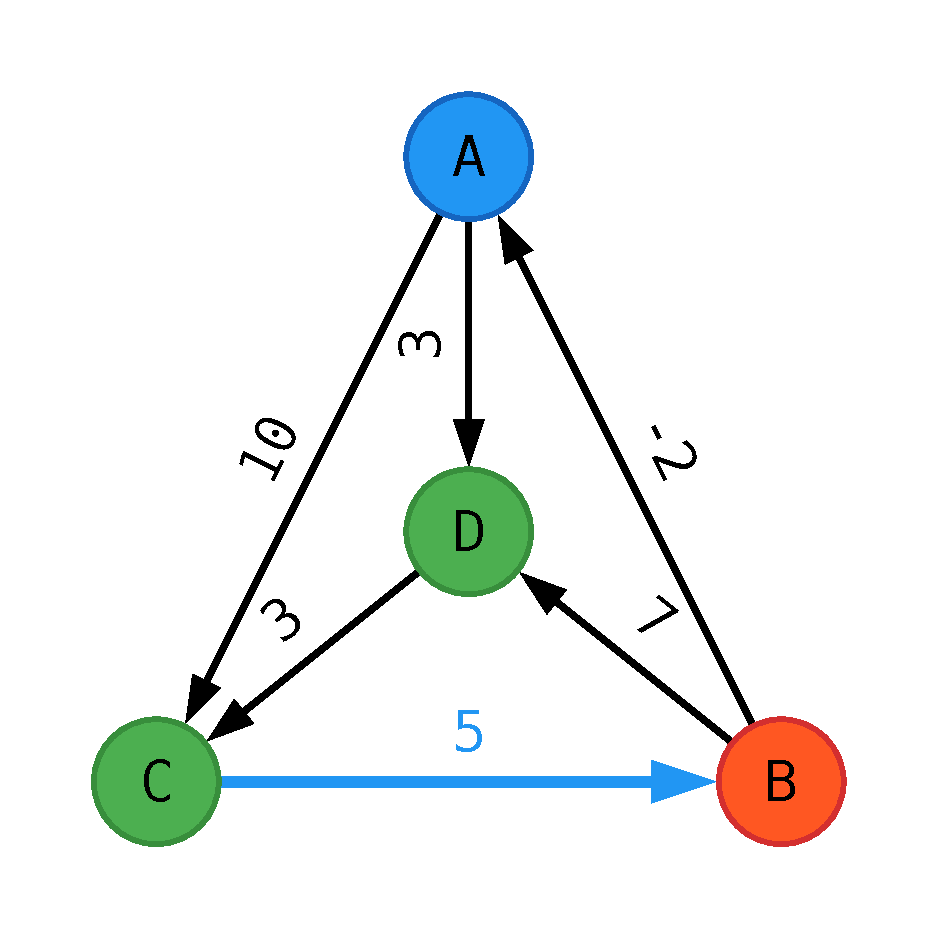
\includegraphics[width=0.28\textwidth]{python/lec13/bellman_ford/bellman_ford-3.pdf}\\[2pt]{\scriptsize Шаг 3}} &
\shortstack{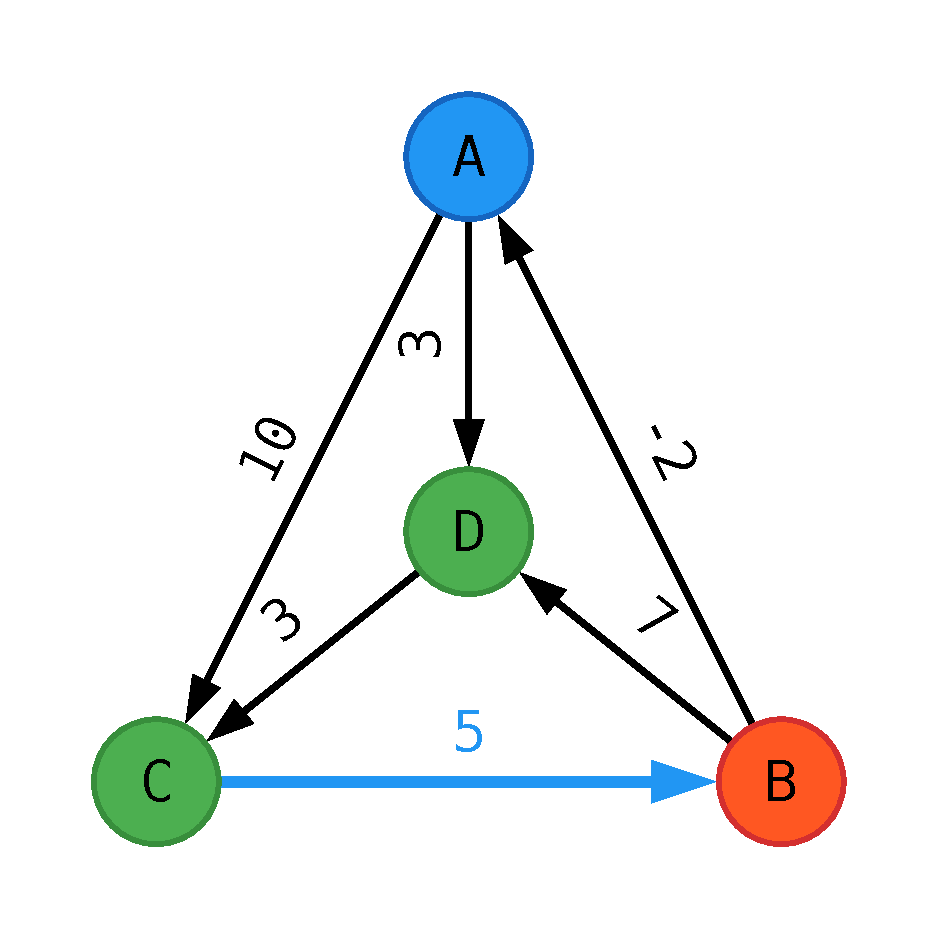
\includegraphics[width=0.28\textwidth]{python/lec13/bellman_ford/bellman_ford-4.pdf}\\[2pt]{\scriptsize Шаг 4}} \\
\end{tabular}\end{center}

\end{algo}

% ===========================================================
%  Алгоритм Флойда-Уоршелла
% ===========================================================

\begin{algo}{Алгоритм Флойда-Уоршелла}{floyd-warshall}

\textbf{Задача} $\odot$: кратчайшие пути для каждой пары $u, v \in V$.

\textbf{Идея:} аналог алгоритма Уоршелла (транзитивное замыкание), но для взвешенного графа.

\textbf{Инициализация:} Матрица $\mu(u, w)$~--- по весам рёбер. Диагональ: $\mu(v,v) = 0$. Нет ребра: $\mu(u,w) = \infty$.

\textbf{Шаг:} $v$~--- ведущая вершина. На $i$-м шаге выделяем $i$-ю строку и $i$-й столбец и смотрим пересечения:

$\forall\, (u, w)$, где $u \neq v$, $w \neq v$:
\[
  \text{если } \mu(u, w) > \mu(u, v) + \mu(v, w), \text{ то }
  \begin{cases}
    \mu(u, w) := \mu(u, v) + \mu(v, w), \\
    P(w) :=
    \begin{cases}
      v, & \text{если } P(v) = \varnothing, \\
      P(v), & \text{если } P(v) \neq \varnothing.
    \end{cases}
  \end{cases}
\]

\textbf{Пример} (рис.~p31-fu-example-1): тот же граф $A, B, C, D$.

\grfig{figures/p31-fu-example-1.pdf}{Алг. Флойда-Уоршелла: тот же граф (BA=-2)}

Шаг~0 (инициализация):
\begin{center}
\begin{tabular}{c|cccc}
     & $A$      & $B$      & $C$      & $D$      \\
\hline
$A$  & 0        & $\infty$ & 10       & 2        \\
$B$  & $-2$     & 0        & $\infty$ & 7        \\
$C$  & $\infty$ & 5        & 0        & $\infty$ \\
$D$  & $\infty$ & $\infty$ & 3        & 0        \\
\end{tabular}
\end{center}

Шаг~1 (ведущая $A$): $\mu(B,C)\colon \infty > (-2)+10 = 8\,(A)$; $\mu(B,D)\colon 7 > (-2)+2 = 0\,(A)$.
\begin{center}
\begin{tabular}{c|cccc}
     & $A$      & $B$      & $C$      & $D$      \\
\hline
$A$  & 0        & $\infty$ & 10       & 2        \\
$B$  & $-2$     & 0        & $8, A$   & $0, A$   \\
$C$  & $\infty$ & 5        & 0        & $\infty$ \\
$D$  & $\infty$ & $\infty$ & 3        & 0        \\
\end{tabular}
\end{center}

Шаг~2 (ведущая $B$): $\mu(C,A)\colon \infty > 5+(-2) = 3\,(B)$; $\mu(C,D)\colon \infty > 5+0 = 5\,(B)$.
\begin{center}
\begin{tabular}{c|cccc}
     & $A$      & $B$      & $C$      & $D$      \\
\hline
$A$  & 0        & $\infty$ & 10       & 2        \\
$B$  & $-2$     & 0        & $8, A$   & $0, A$   \\
$C$  & $3, B$   & 5        & 0        & $5, B$   \\
$D$  & $\infty$ & $\infty$ & 3        & 0        \\
\end{tabular}
\end{center}

Шаг~3 (ведущая $C$): $\mu(A,B)\colon \infty > 10+5 = 15\,(C)$; $\mu(D,A)\colon \infty > 3+3 = 6\,(C)$; $\mu(D,B)\colon \infty > 3+5 = 8\,(C)$.
\begin{center}
\begin{tabular}{c|cccc}
     & $A$      & $B$      & $C$      & $D$      \\
\hline
$A$  & 0        & $15, C$  & 10       & 2        \\
$B$  & $-2$     & 0        & $8, A$   & $0, A$   \\
$C$  & $3, B$   & 5        & 0        & $5, B$   \\
$D$  & $6, C$   & $8, C$   & 3        & 0        \\
\end{tabular}
\end{center}

Шаг~4 (ведущая $D$): $\mu(A,B)\colon 15 > 2 + 8 = 10\,(D)$ --- путь $A \to D \to C \to B$; $\mu(A,C)\colon 10 > 2+3 = 5\,(D)$; $\mu(B,C)\colon 8 > 0+3 = 3\,(A)$ --- путь $B \to A \to D \to C$, первая путевая точка $A$.
\begin{center}
\begin{tabular}{c|cccc}
     & $A$      & $B$      & $C$      & $D$      \\
\hline
$A$  & 0        & $10, D$  & $5, D$   & 2        \\
$B$  & $-2$     & 0        & $3, A$   & $0, A$   \\
$C$  & $3, B$   & 5        & 0        & $5, B$   \\
$D$  & $6, C$   & $8, C$   & 3        & 0        \\
\end{tabular}
\end{center}

\textbf{Восстановление:}
$A \to D$: путевая точка не записана (прямое ребро), путь $A \to D$,
длина $= 2$.
$C \to B$: путевая точка тоже не записана --- кратчайший путь так и
остался прямым ребром $C \to B$ длины $5$ (обходы $C \to A \to \ldots$
дороже: $\mu(C,A) = 3$, а ребра $A \to B$ нет, $\mu(A,B) = 10$).
$A \to B$: $P_{AB} = D$, далее $\mu(D, B)$: $P_{DB} = C$, далее прямое
ребро $C \to B$; итог $A \xrightarrow{2} D \xrightarrow{3} C
\xrightarrow{5} B$, длина $= 10$.

\textbf{Циклы отрицательного суммарного веса} $\Leftrightarrow$ отрицательные значения на главной диагонали.

\end{algo}

% ============================================================
\begin{task}{Кратчайшие пути: алгоритм Дейкстры}{dijkstra-task}
\textbf{Условие.} Дан неориентированный взвешенный граф на вершинах
$S,A,B,C,D,F$ с рёбрами
\[
  SA=2,\ SB=5,\ AB=1,\ AC=4,\ BD=3,\ CD=1,\ CF=6,\ DF=2.
\]
Найдите кратчайшие расстояния от вершины $S$ до всех остальных алгоритмом Дейкстры.

\smallskip
\grfig[0.42]{python/03-dijkstra/3-dijkstra-0.pdf}{Граф задачи (условие)}

\textbf{Решение.} Дейкстра поддерживает множество вершин с окончательно
найденным расстоянием. На каждом шаге фиксируется вершина с наименьшей текущей
оценкой $d$, после чего релаксируются её рёбра.
\begin{enumerate}
  \item Старт: $d[S]=0$, остальные $=\infty$. Фиксируем $S$:
        $d[A]=2,\ d[B]=5$.
  \item Минимум среди нефиксированных --- $A\,(2)$. Фиксируем $A$:
        $d[B]=\min(5,\,2+1)=3$, $d[C]=2+4=6$.
  \item Минимум --- $B\,(3)$. Фиксируем $B$: $d[D]=3+3=6$.
  \item Минимум --- $C\,(6)$. Фиксируем $C$: $D$ ($6+1=7>6$ --- без изменений),
        $d[F]=6+6=12$.
  \item Минимум --- $D\,(6)$. Фиксируем $D$: $d[F]=\min(12,\,6+2)=8$.
  \item Фиксируем $F\,(8)$. Все вершины обработаны.
\end{enumerate}

%% [серия шагов перенесена в раздел алгоритма]

\textbf{Ответ.} $d[S]=0,\ d[A]=2,\ d[B]=3,\ d[C]=6,\ d[D]=6,\ d[F]=8$.
\end{task}

% ============================================================
\begin{task}{Кратчайшие пути с отрицательными рёбрами: Форд—Беллман}{bellman-task}
\textbf{Условие.} Дан \emph{ориентированный} взвешенный граф на вершинах
$S,A,B,C,D,F$ с дугами
\[
  S\!\to\!A=3,\ S\!\to\!B=2,\ A\!\to\!C=2,\ B\!\to\!A=-2,\
  C\!\to\!D=1,\ B\!\to\!D=5,\ D\!\to\!F=3,\ C\!\to\!F=6.
\]
Найдите кратчайшие расстояния от $S$ алгоритмом Форда—Беллмана.

\smallskip
\grfig[0.42]{python/04-bellman-ford/4-bellman-ford-0.pdf}{Граф задачи (условие)}

\textbf{Решение.} Форд—Беллман выполняет до $|V|-1$ итераций, на каждой
релаксируя все дуги; отрицательные веса допустимы (при отсутствии отрицательных
циклов).
\begin{itemize}
  \item \textbf{Итерация 1.} $d[A]=3,\ d[B]=2,\ d[C]=5$; затем дуга
        $B\!\to\!A$ улучшает $d[A]=2-2=0$; далее $d[D]=6,\ d[F]=9$.
  \item \textbf{Итерация 2.} Так как $d[A]$ упало до $0$, пересчёт даёт
        $d[C]=0+2=2$, $d[D]=2+1=3$, $d[F]=3+3=6$.
  \item \textbf{Итерация 3.} Изменений нет --- расстояния стабилизировались.
\end{itemize}
Заметим: кратчайший путь до $A$ идёт \emph{не} напрямую $S\!\to\!A$ (вес $3$),
а через $S\!\to\!B\!\to\!A$ (вес $2+(-2)=0$). Именно из-за отрицательной дуги
здесь нужен Форд—Беллман, а не Дейкстра.

%% [серия шагов перенесена в раздел алгоритма]

\textbf{Ответ.} $d[S]=0,\ d[A]=0,\ d[B]=2,\ d[C]=2,\ d[D]=3,\ d[F]=6$.
\end{task}
